\documentclass[11pt]{article}

\usepackage[a4paper,
            bindingoffset=0.5cm,
            left=3cm,
            right=3cm,
            top=3cm,
            bottom=4cm,
            footskip=1.5cm]{geometry}
            
%
\usepackage[T1]{fontenc}
\usepackage{graphicx}
\usepackage{enumitem}
\usepackage{blindtext}
\usepackage{float}
%

\setcounter{secnumdepth}{3}

%%%%%%%%%%%%%%%%%%%%%
\title{\textbf{Critical Systems Lab - MESCC\\ Water Pumping Automated System}}
\date{ISEP, January 2024}
\author{Ricardo Mendes\\ 1201779
\and Arthur Gerbelli\\ 1220201}
%%%%%%%%%%%%%%%%%%%%%

\begin{document}

\maketitle              
\newpage
\tableofcontents
\newpage

%
\section{Introduction}

\section{Requirement Specification}

%%%
\subsection{Problem Domain}

%%%
\subsubsection{Stakeholder Needs}

\begin{enumerate}[leftmargin=4em, font=\small, label=\textbf{SN-\arabic*}]
	\setlength\itemsep{.5em}
	\item 
		\begin{enumerate}[leftmargin=1.5em, font=\small, label=\textbf{.\arabic*:}]
		\setlength\itemsep{0em}	
		\item The water in the wet well must be pumped to a higher level.
		\item Every WPS is an independent system; they don't have influence on each other.
		\end{enumerate}
	\item 
		\begin{enumerate}[leftmargin=1.5em, font=\small, label=\textbf{.\arabic*:}]
		\setlength\itemsep{0em}	
		\item The status of each element of the wet well needs to be displayed in a Remote Status Station (RSS). 
		\item The RSS must display the water level, the pump status, an alarme and a button to disable the alarm.
		\end{enumerate}
		
	\item The status information must be accessible through a web page.
\end{enumerate}

%%%
\subsubsection{System Context}

\begin{figure}[H]
  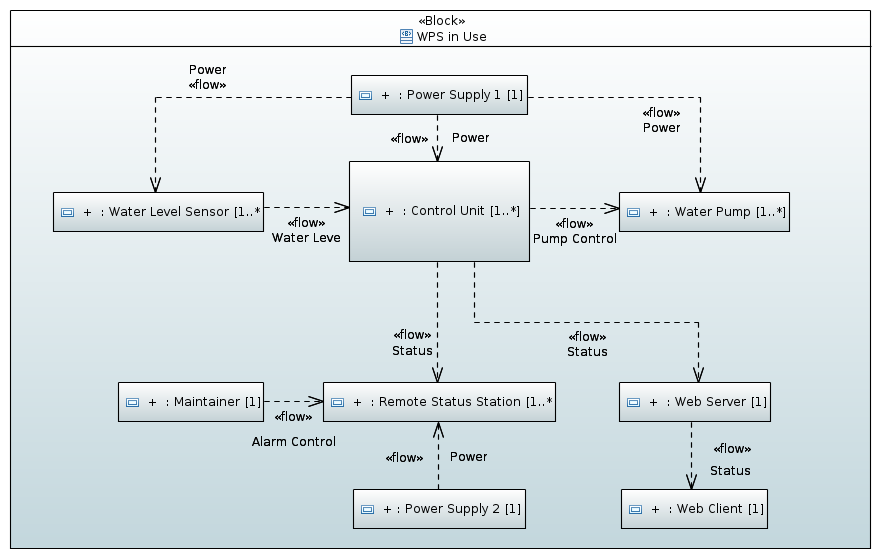
\includegraphics[width=300px]{../diagrams/system-context-01.png}
  \caption{System Context}
  \label{fig:System Context}
\end{figure}	

%%%
\subsubsection{Use Cases}
By analyzing stakeholder needs, we can see that the main goal of the WPS is to control the water level inside the wet well. This goal can be captured in the model as
the Control Water Level use case of the Control Unit In Use system context. 

\begin{figure}[H]
  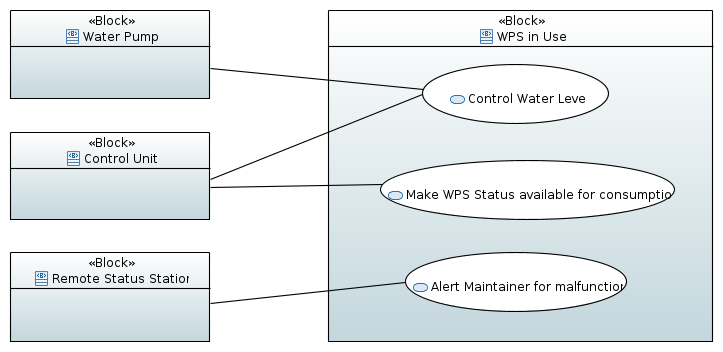
\includegraphics[width=300px]{../diagrams/use-cases-01.png}
  \caption{Use Case diagram}
  \label{fig:Use Case1}
\end{figure}

\begin{figure}[H]
  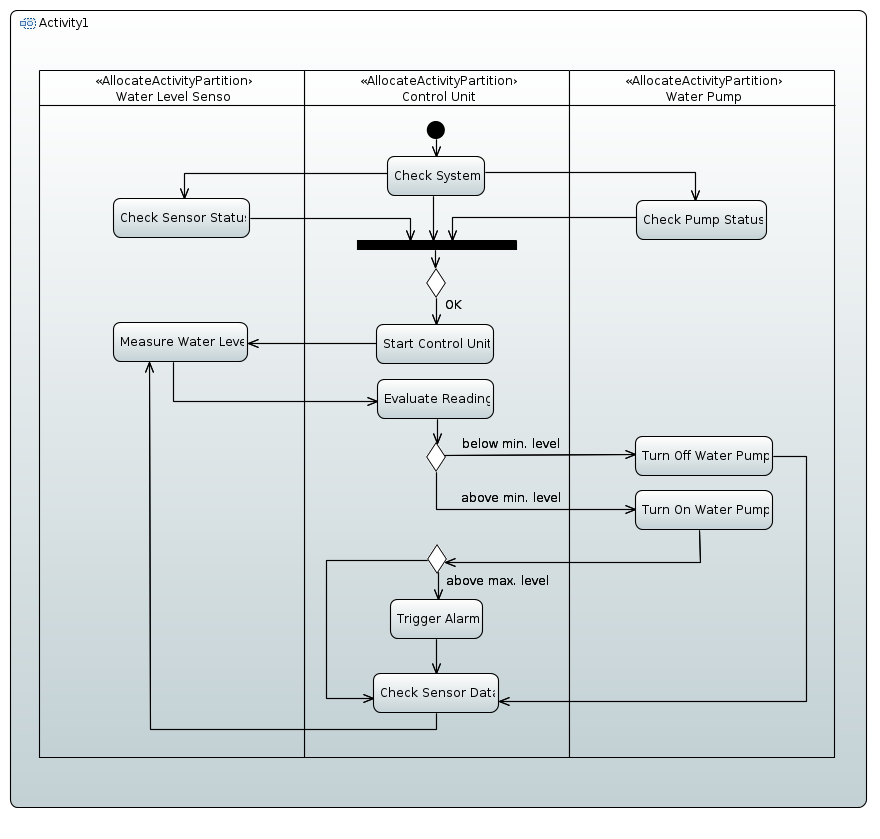
\includegraphics[width=300px]{../diagrams/use-case-activity-diagram-01.png}
  \caption{Use Case Activity diagram}
  \label{fig:Use Case2}
\end{figure}

%%%
\subsubsection{Measure of Effectiveness}

\begin{figure}[H]
  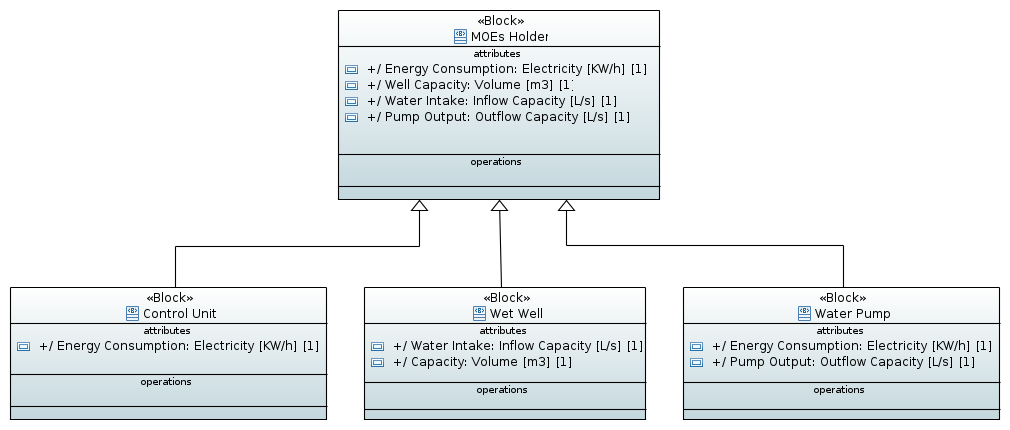
\includegraphics[width=300px]{../diagrams/measure-of-effectiveness.png}
  \caption{Measure of Effectiveness diagram}
  \label{fig:MoE}
\end{figure}

%%%
\subsubsection{Functional Analysis}

\begin{figure}[H]
  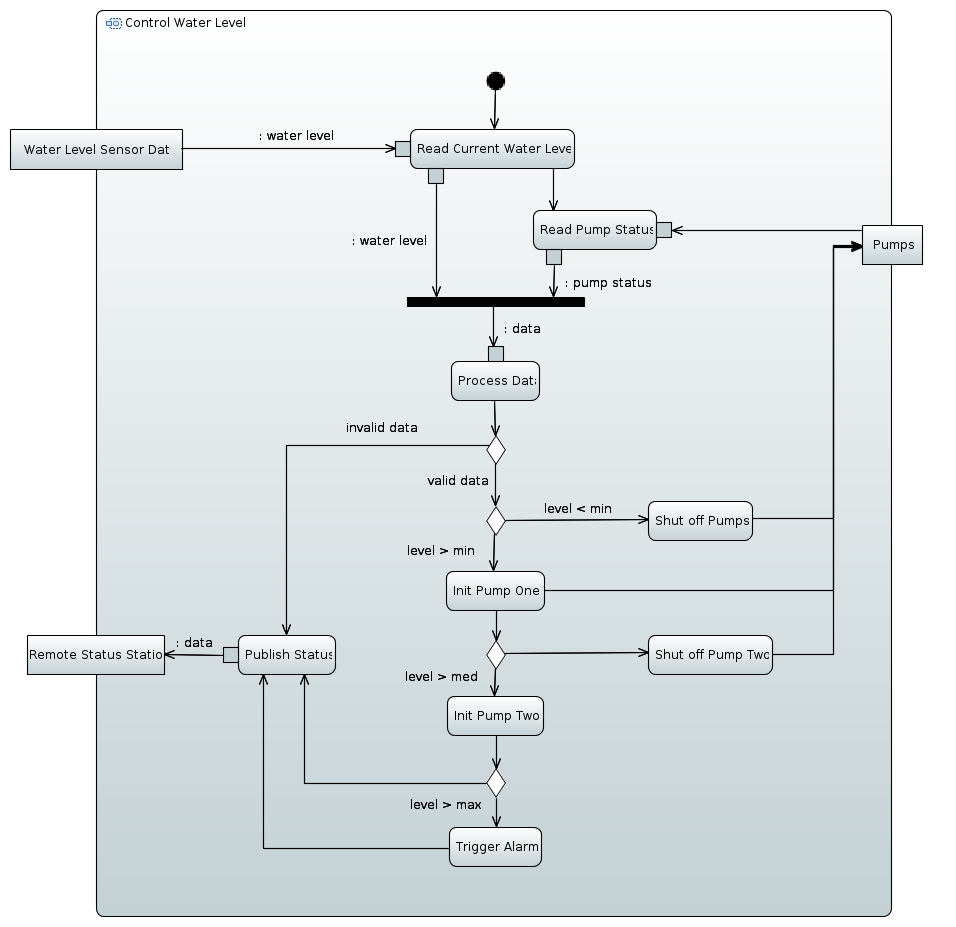
\includegraphics[width=300px]{../diagrams/functional-analysis-wps.png}
  \caption{Functional Analysis diagram}
  \label{fig:Functional Analysis}
\end{figure}

%%%
\subsubsection{Conceptual Subsystems}

\begin{figure}[H]
  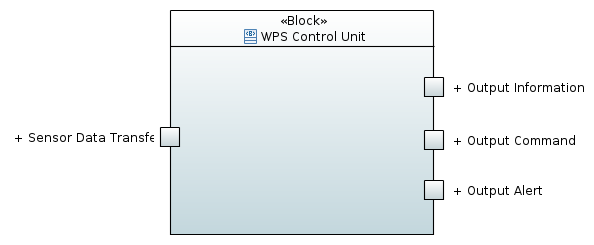
\includegraphics[width=300px]{../diagrams/conceptual-subsystem-communication-wps.png}
  \caption{Conceptual Subsystem Communication diagram}
  \label{fig:Conceptual Subsystem}
\end{figure}

%%%
\subsubsection{Traceability to Stakeholder}

%%%
\subsection{Solution Domain}

%%%
\subsubsection{System Requirements}

\begin{enumerate}[leftmargin=4em, font=\small, label=\textbf{SR-\arabic*}]
	\setlength\itemsep{.5em}
	\item 
		\begin{enumerate}[leftmargin=1.5em, font=\small, label=\textbf{.\arabic*:}]
		\setlength\itemsep{0em}
		\item While the water level is above the minimum level, WPS shall have a pump working.
		\item When the water level is below minimum level, WPS shall have all pumps stopped.
		\item If the water level is above the maximum level, then the WPS shall trigger an alarm at the Remote Status Station (RSS).
		\item A second pump shall be turned on only when the water level is above 2/3 the maximum water level.
		\item When only one pump is available, the maximum water level shall be reduced to 2/3.
		\end{enumerate}
	\item
		\begin{enumerate}[leftmargin=1.5em, font=\small, label=\textbf{.\arabic*:}]s
		\setlength\itemsep{0em}
		\item The status of all WPS shall be displayed on all RSS.
		\item If the alarm is ON, the button in the RSS shall only disable it.
		\end{enumerate}
	\item The status of all WPS shall be visible on one web page.

\end{enumerate}

%%%
\subsubsection{System Structure}

\begin{figure}[H]
  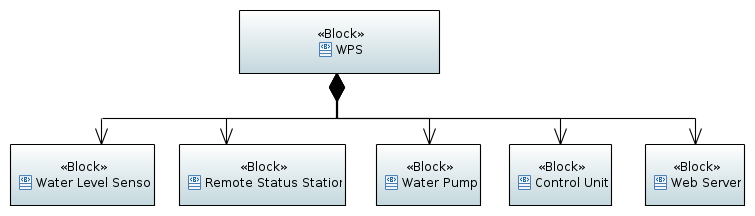
\includegraphics[width=300px]{../diagrams/system-structure.png}
  \caption{System Structure Diagram}
  \label{fig:System Structure Diagram}
\end{figure}

%%%
\subsubsection{System Behavior}

\begin{figure}[H]
  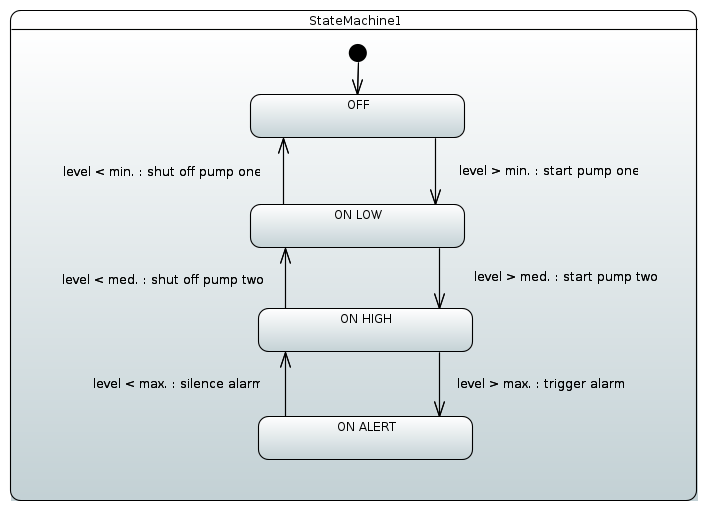
\includegraphics[width=300px]{../diagrams/state-machine-wps.png}
  \caption{State Machine}
  \label{fig:State Machine}
\end{figure}

%%%
%%%
%%%
\subsection{Analysis of safety and reliability}

\begin{enumerate}[leftmargin=4em, font=\small, label=\textbf{H-\arabic*:}]
	\setlength\itemsep{.5em}
	\item 
		\begin{itemize}
		\setlength\itemsep{0em}
        		\item \textbf{Description:} One of the pumps stops working.
		\item Cause: Mechanical problem.
    		\item Effect: Lost of redundancy and reduction of system performance.
    		\item \textbf{Mitigation:} Reduce the maximum water level to 2/3 and trigger alarm.
		\end{itemize}
	\item 
		\begin{itemize}
		\setlength\itemsep{0em}
    		\item \textbf{Description:} The two level sensors give contradictory readings, i.e. one above max and one below min.
		\item Cause: Sensor malfunction, connection issues.
    		\item Effect: Inapropriete system behavior. 
    		\item \textbf{Mitigation:} Choose a worst case or compare with the last reading to find the fault. Trigger alarm.
		\end{itemize}
	\item 
		\begin{itemize}
		\setlength\itemsep{0em}
    		\item \textbf{Description:} Power shortage.
		\item Cause: Multiple causes
    		\item Effect: Complete failure of the system.
    		\item \textbf{Mitigation:} RSS with independente power supply and trigger alarm.
		\end{itemize} 
	\item 
		\begin{itemize}
		\setlength\itemsep{0em}
    		\item \textbf{Description:} Both pumps stopped working.
		\item Cause: Mechanical problem.
    		\item Effect: Complete failure of the system.
    		\item \textbf{Mitigation:} Trigger alarm.
		\end{itemize} 
	\item 
		\begin{itemize}
		\setlength\itemsep{0em}
    		\item \textbf{Description:} RSS are not getting information from WPS.
		\item Cause: Connection issues or Messagem broker stoped working.
    		\item Effect: Wrong status readings.
    		\item \textbf{Mitigation:} Trigger alarm or remove broker as single point of failure by using protocols like DDS.
		\end{itemize} 
	\item 
		\begin{itemize}
		\setlength\itemsep{0em}
    		\item \textbf{Description:} RSS stops working.
		\item Cause: Malfunction.
    		\item Effect: Unknown WPS status.
    		\item \textbf{Mitigation:} Have redundancy by having multiple RSS and each one displaying all statuses from all WPS.
		\end{itemize} 
	\item 
		\begin{itemize}
		\setlength\itemsep{0em}
    		\item \textbf{Description:} A pump doesn't turn OFF when the water level in bellow minimum.
		\item Cause: Mechanical problem.
    		\item Effect: Pump overheating and complete failure.
    		\item \textbf{Mitigation:} Trigger alarm.
		\end{itemize} 
\end{enumerate}

%%%
\section{Selected Technologies}

\begin{figure}[H]
  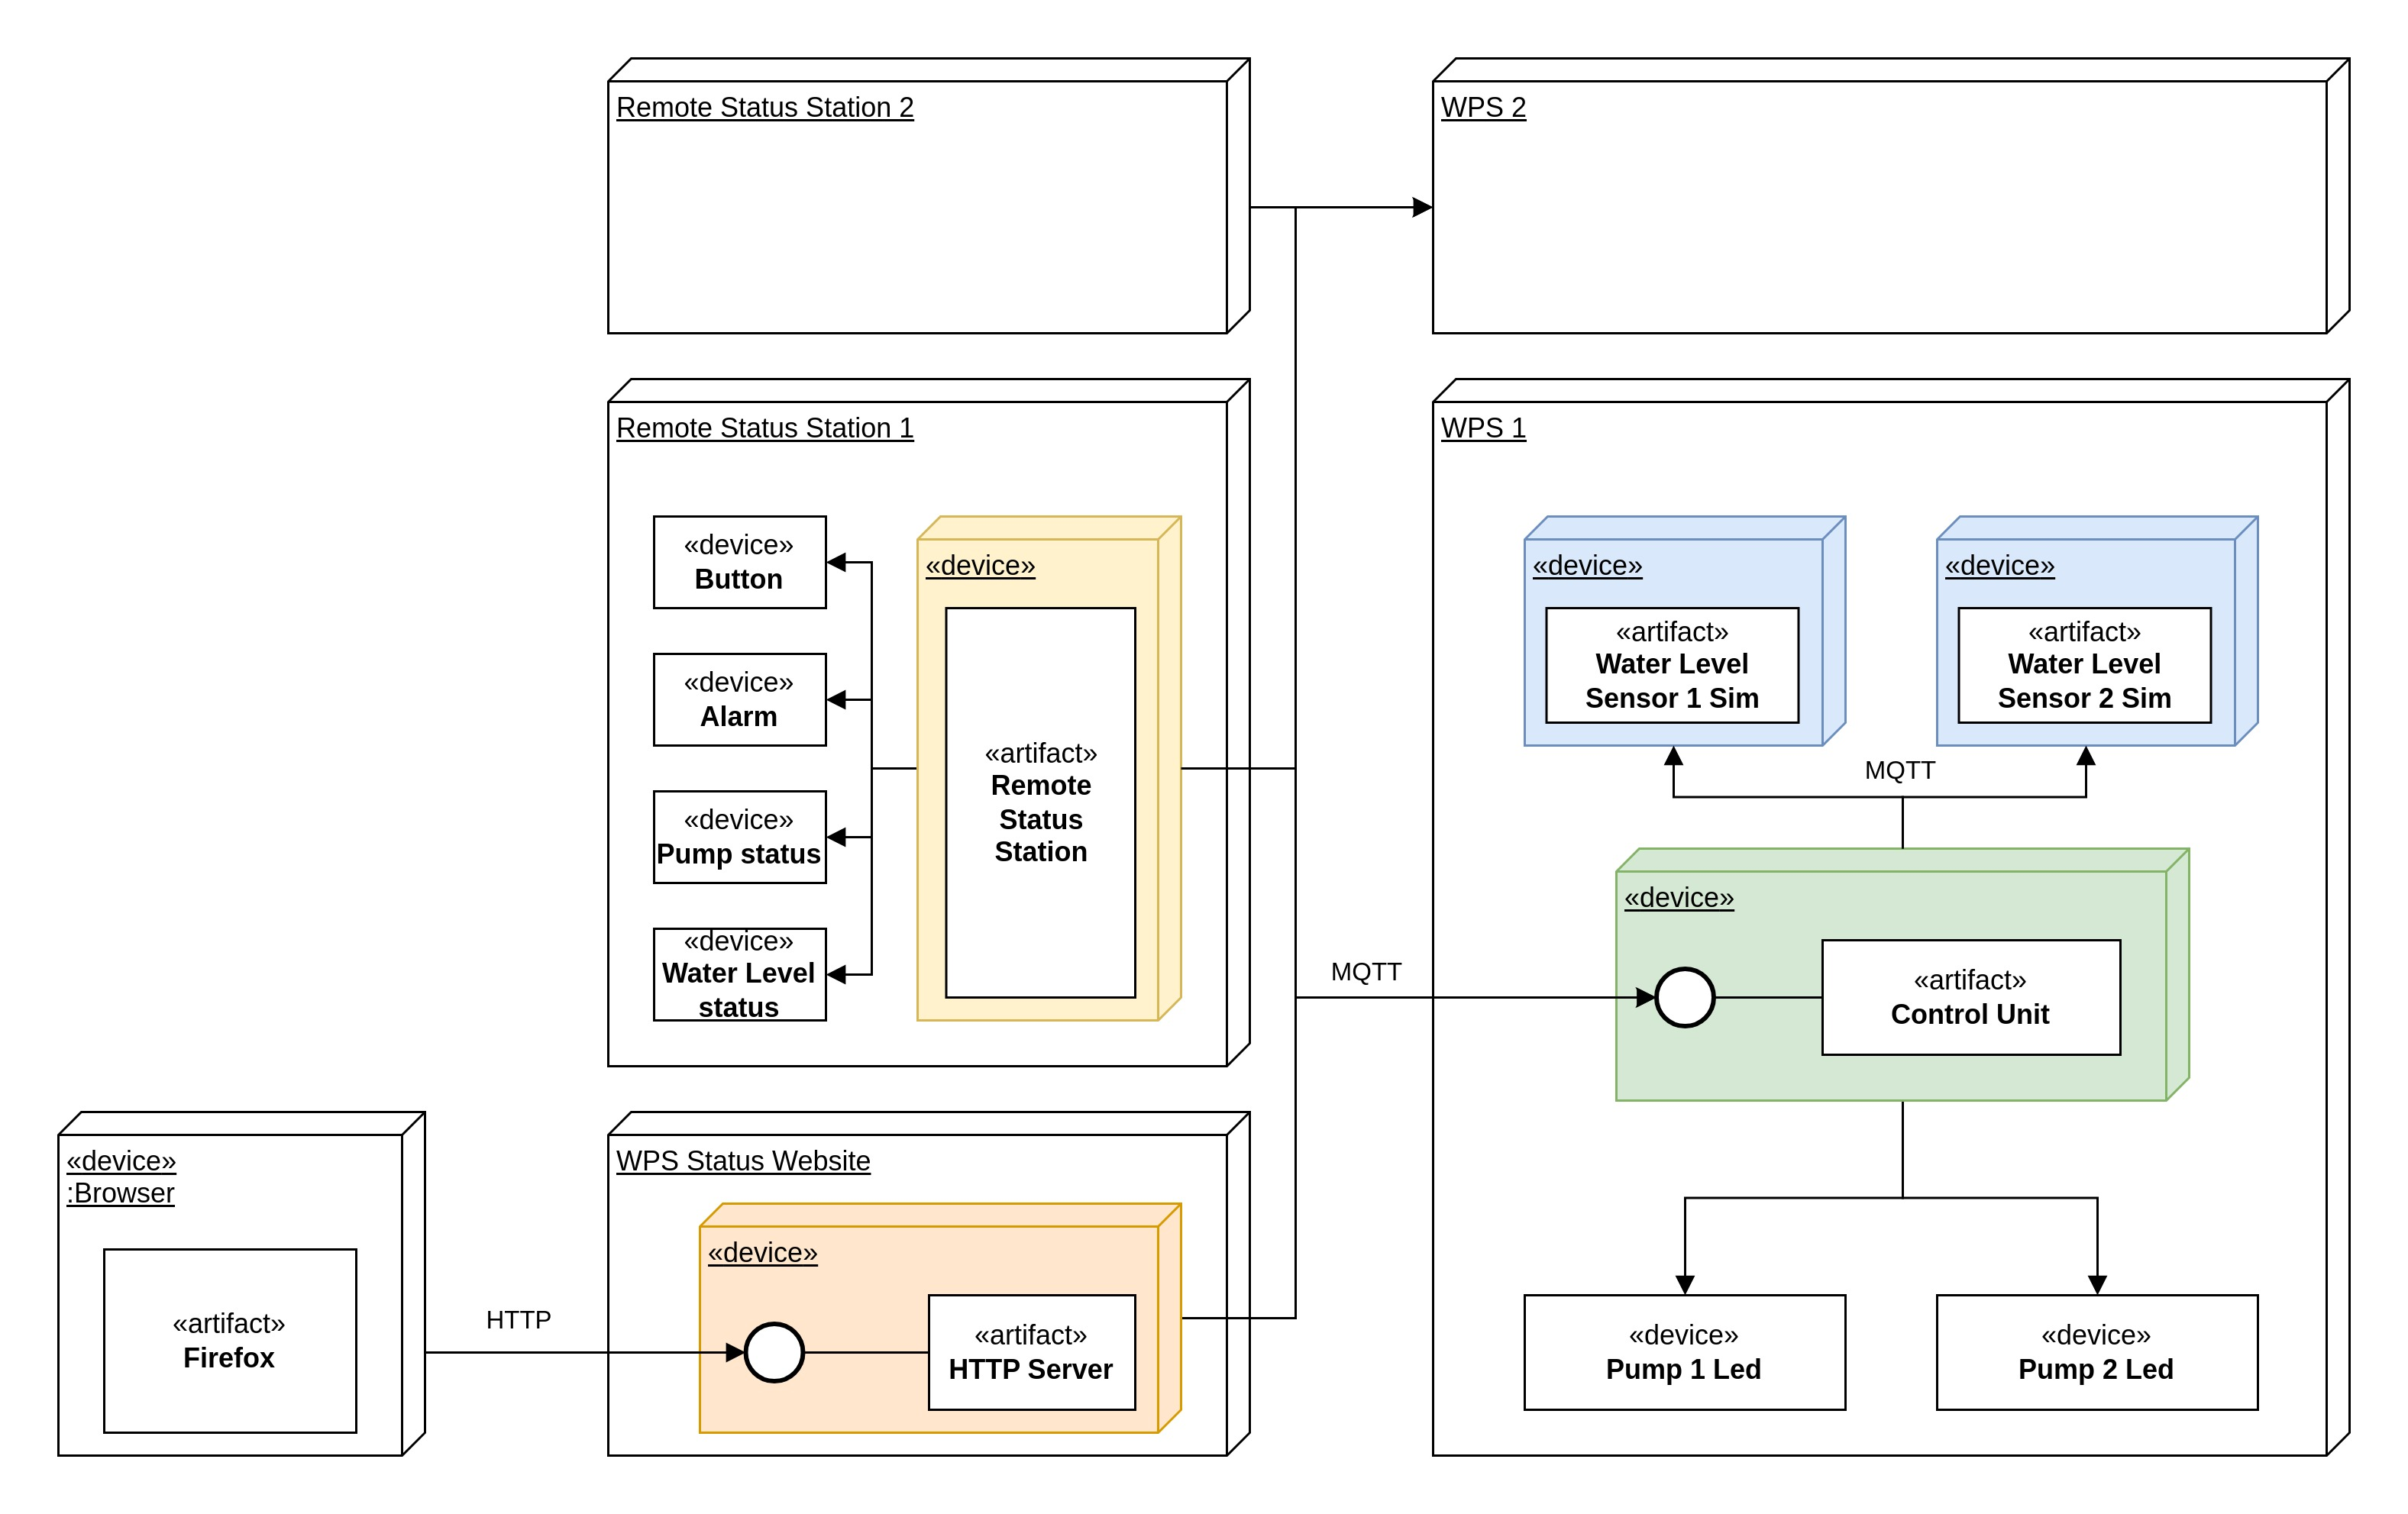
\includegraphics[width=300px]{../diagrams/deployment-diagram-WPS.jpg}
  \caption{Deployment diagram}
  \label{fig:Deployment Diagram}
\end{figure}

%%%
\section{List of physical sensors/actuators}

\begin{figure}[H]
  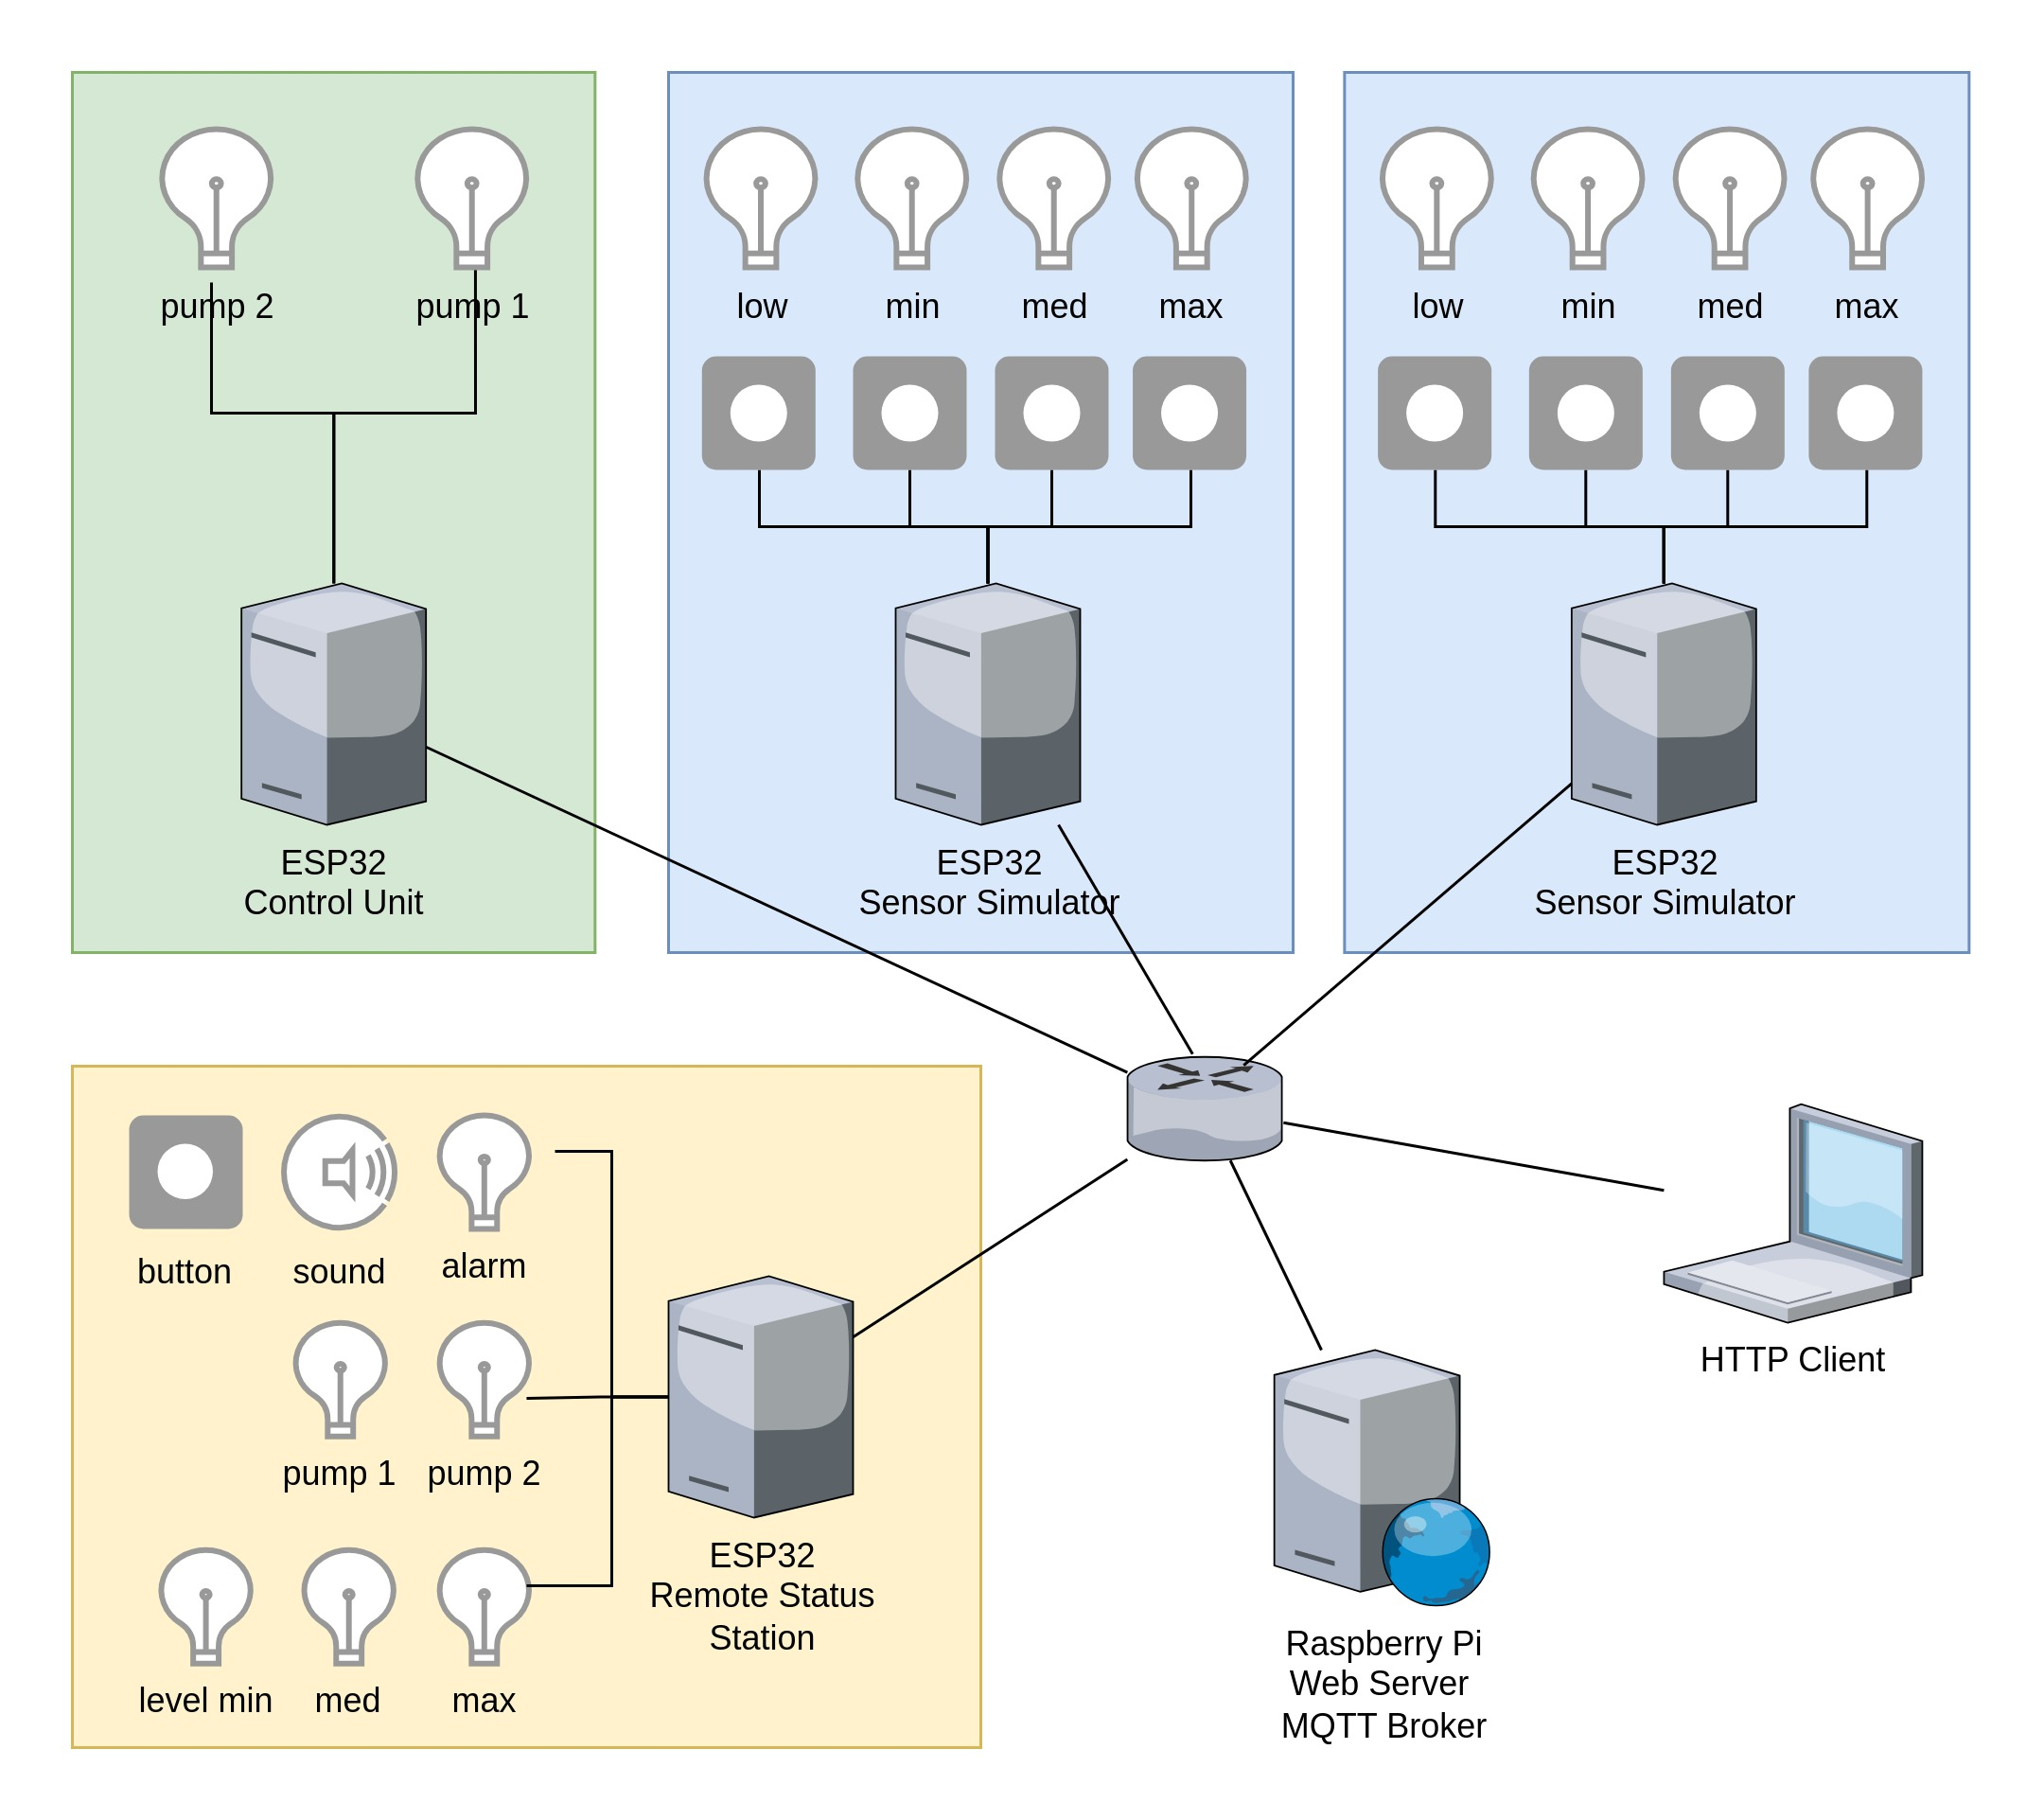
\includegraphics[width=300px]{../diagrams/network-diagram-WPS.jpg}
  \caption{Network diagram}
  \label{fig:Network1 Diagram}
\end{figure}

\end{document}
